\documentclass[a4paper, 12pt]{article}
\usepackage{eurosym}
\usepackage{pdflscape}
\usepackage{pgfgantt}
\usepackage{pgfplots}
\usepackage{booktabs}
\usepackage{longtable}


\newcommand{\templates}{../../template}
\usepackage[a4paper, margin=2.5cm]{geometry}

\usepackage{enumitem}
\setlist[itemize]{noitemsep}
\setlist[enumerate]{noitemsep}

\let\oldpar\paragraph
\renewcommand{\paragraph}[1]{\oldpar{#1\\}\noindent}

% Avoid dots in the table of contents, it mess with the gulpease calculation
\makeatletter
\renewcommand{\@dotsep}{10000} 
\makeatother
\usepackage{graphicx}
\usepackage{hyperref}
\usepackage{makecell}
\usepackage{fancyhdr}

\newcommand{\settitolo}[1]{\newcommand{\titolo}{#1\\}}
\newcommand{\setprogetto}[1]{\newcommand{\progetto}{#1\\}}
\newcommand{\setcommittenti}[1]{\newcommand{\committenti}{#1\\}}
\newcommand{\setredattori}[1]{\newcommand{\redattori}{#1\\}}
\newcommand{\setrevisori}[1]{\newcommand{\revisori}{#1\\}}
\newcommand{\setresponsabili}[1]{\newcommand{\responsabili}{#1\\}}
\newcommand{\setversione}[1]{
	\ifdefined\versione\renewcommand{\versione}{#1\\}
	\else\newcommand{\versione}{#1\\}\fi
}
\newcommand{\setdestuso}[1]{\newcommand{\uso}{#1\\}}
\newcommand{\setdescrizione}[1]{\newcommand{\descrizione}{#1\\}}

\newcommand{\makefrontpage}{
	\begin{titlepage}
		\begin{center}

		
\includegraphics[width=0.4\textwidth]{\templates/4ourSquared_logo}\\

		{\Large 4OURSQUARED}\\[6pt]
		\href{mailto://4oursquared.unipd@gmail.com}{4oursquared.unipd@gmail.com}\\
		
		\ifdefined\progetto
		\vspace{1cm}
		{\Large\progetto}
		{\large\committenti}
		\else\fi
		
		\vspace{1.5cm}
		{\LARGE\titolo}
		
		\vfill
		
		\begin{tabular}{r | l}
		\multicolumn{2}{c}{\textit{Informazioni}}\\
		\hline
		
		\ifdefined\redattori
			\textit{Redattori} &
			\makecell[l]{\redattori}\\
		\else\fi
		\ifdefined\revisori
			\textit{Revisori} &
			\makecell[l]{\revisori}\\
		\else\fi
		\ifdefined\responsabili
			\textit{Responsabili} &
			\makecell[l]{\responsabili}\\
		\else\fi
		
		\ifdefined\versione
			\textit{Versione} & \versione
		\else\fi
		
		\textit{Uso} & \uso
		
		\end{tabular}
		
		\vspace{2cm}
		
		\ifdefined\descrizione
		Descrizione
		\vspace{6pt}
		\hrule
		\descrizione
		\else\fi
		\end{center}
	\end{titlepage}
}
\usepackage{hyperref}
\usepackage{array}
\usepackage{tabularx}
\usepackage{adjustbox}

\newcounter{verscount}
\setcounter{verscount}{0}
\newcommand{\addversione}[5]{
	\ifdefined\setversione
		\setversione{#1}
	\else\fi
	\stepcounter{verscount}
	\expandafter\newcommand%
		\csname ver\theverscount \endcsname{#1&#2&#3&#4&#5}
}

\newcommand{\listversioni}{
	\ifnum\value{verscount}>1
		\csname ver\theverscount \endcsname
		\addtocounter{verscount}{-1}
		\\\hline
		\listversioni
	\else
		\csname ver\theverscount \endcsname\\\hline
	\fi
}

\newcommand{\makeversioni}{
	\begin{center}
		\begin{tabularx}{\textwidth}{|c|c|c|c|X|}
		\hline
		\textbf{Versione} & \textbf{Data} & \textbf{Redattore} & \textbf{Verificatore} & \textbf{Descrizione} \\
		\hline
		\listversioni
		\end{tabularx}
	\end{center}
	\clearpage
}
\graphicspath{ {./immagini/} }

\settitolo{Analisi dei requisiti}
\setredattori{Nicolas Alberti \\ Romina Brotto \\ Erica Cavaliere \\ Francesco Ceccato }
\setdestuso{esterno}
\setdescrizione{
Questo documento si occupa di riportare un'analisi di tutti gli elementi richiesti e i vincoli da rispettare per una completa comprensione del progetto.
}


\addversione{0.0.1}{05/05/2023}{Erica Cavaliere}{Lorenzo Salami}{Stesura iniziale}
\addversione{0.0.2}{05/05/2023}{Francesco Ceccato}{Lorenzo Salami}{Inserimento di alcuni casi d'uso}
\addversione{0.0.3}{09/05/2023}{Brotto Romina}{Soldà Matteo}{Aggiunta sezioni 2, 2.1, 4, 4.1 ed inizio stesura requisiti funzionali}
\addversione{0.0.4}{10/05/2023}{Alberti Nicolas}{Brotto Romina}{}

\def\pgfcalendarmonthitname#1{%
\ifcase#1 \or Gennaio\or Febbraio\or Marzo\or Aprile\or Maggio\or Giugno\or Luglio\or Agosto\or Settembre\or Ottobre\or Novembre\or Dicembre\fi%
}
\usepgfplotslibrary{dateplot}

\begin{document}
\makeindexdetails
\makefrontpage \makeversioni
\tableofcontents
\newpage
\clearpage
\makecontentsdetails{Analisi dei requisiti} 

\section{Introduzione}
\subsection{Scopo del Documento}
In questo progetto viene richiesto di creare un sistema che permetta di gestire i lampioni, accendendo una o più luci se sono presenti nelle vicinanze una o più persone o spegnendole altrimenti.\newline
Bisognerà che ci sia anche un modo per registrare i guasti degli impianti e segnalarli tramite apposita applicazione.

\subsection{Riferimenti}
\subsubsection*{Riferimenti normativi}
\begin{itemize}
    \item Capitolato d'appalto: C2; 
    \item Norme di Progetto.
\end{itemize}

\subsubsection*{Riferimenti informativi}
\begin{itemize}
    \item Slide analisi dei requisiti - Materiale didattico del corso IS;
    \item Slide diagrammi dei casi d'uso - Materiale didattico del corso IS.
\end{itemize}
\newpage
\section{Descrizione del Prodotto}
L'azienda \textit{Imola Informatica} propone attraverso il capitolato C2:
\textit{Lumos Minima}. L'obiettivo è sviluppare un sistema per l'ottimizzazione
dell'illuminazione pubblica che permetta ai gestori di sfruttare la possibilità
di regolare l'intensità di luce emessa dagli impianti, grazie all'utilizzo di
sensori specifici che permettono di ottenere informazioni legate all'ambiente circostante.
\subsection{Scopo del Prodotto}
Il sistema sopra citato consentirebbe di garantire sicurezza stradale e sociale, e al tempo stesso permetterebbe di risparmiare energia e quindi risorse economiche ed ambientali. Il processo è caratterizzato da operazioni effettuate dal sistema e/o dai gestori:
\begin{itemize}
    \item Rilevamento della presenza di persone in prossimità della fonte luminosa;
    \item Aumento e riduzione dell'intensità luminosa;
    \item Rilevamento automatico del guasto di un impianto di illuminazione;
    \item Segnalazione manuale del guasto di un impianto di illuminazione;
    \item Aumento e riduzione manuale dell'intensità luminosa;
    \item Inserimento e gestione di un impianto luminoso;
    \item Aumento o riduzione globale dell'intensità luminosa. 
\end{itemize}

\subsection{Parti del Prodotto}
Il prodotto si compone delle seguenti parti: % BOZZA
\begin{itemize}
    \item Landing page per permettere l'autenticazione dell'operatore;
    \item Web App con dashboard per visualizzare, selezionare tutti i gruppi di
    impianti luminosi ed interagire con essi.
\end{itemize}
% BOZZA - DA DEFINIRE
Per ogni impianto luminoso deve essere prevista una modalità a funzionamento
automatico ed una modalità a funzionamento manuale, in cui l'operatore potrà
configurare a proprio piacimento gli elementi dell'impianto. 
\subsection{Caratteristiche utenti}
La Web App prevede due tipologie di utenti:
\begin{itemize}
    \item operatore non autenticato, che può: \begin{itemize}
        \item visualizzare la landing page;
        \item accedere al servizio previo possesso di credenziali autenticate.
    \end{itemize}
    \item operatore autenticato, che può: \begin{itemize}
        \item visualizzare tutti gli impianti luminosi gestiti dall'organizzazione;
        \item interagire con ogni impianto e modificarne il funzionamento;
        \item visualizzare eventuali errori e/o guasti.
    \end{itemize}
\end{itemize}
% BOZZA - DA DEFINIRE
Il prodotto si rivolge a tutte le organizzazioni che necessitano di gestire un
numero consistente di impianti luminosi, a loro volta composti da più elementi
quali luci e sensori. L'utente finale deve conoscere il funzionamento di tali
componenti, al fine di poter gestire nella maniera più adeguata gli impianti ed
inoltre deve saper interpretare gli errori forniti dal prodotto, per poter
correggere il funzionamento dell'impianto.

\subsection{Vincoli e preferenze}
Il proponente non impone particolari vincoli nella scelta delle tecnologie e dei linguaggi, sono stati però forniti alcui suggerimenti da prendere in considerazione:
\begin{itemize}
    \item utilizzo di React per lo sviluppo delle parti di Front-end;
    \item utilizzo di Node JS per lo sviluppo delle parti di Back-end;
\end{itemize}

Per il completamento del progetto il proponente richiede che siano ottenuti i
seguienti risultati:
\begin{itemize}
    \item applicazione Web Responsive che soddisfi i requisiti obblgatori
    illustrati dai casi d'uso;
    \item test che dimostrino il corretto funzionamento dei servizi e delle
    funzionalità previste, con una copertura minima dell'80\%;
    \item documentazione sulle scelte implementative e progettuali con le
    motivazioni e i problemi aperti ed eventuali soluzioni da esplorare.
\end{itemize}
Sono di interesse altri due risultati desiderabili ma non vincolanti al fine del
completamento del progetto:
\begin{itemize}
    \item cifratura di tutte le comunicazoni fra App e Server per garantire la
    validità delle informazioni;
    \item analisi riguardante sia il carico massimo supportato in numero di
    dispositivi che del servizio cloud più adatto per supportarlo
    analizzando prezzo, stabilità, del servizio ed assistenza.
\end{itemize} 
\newpage
\section{Casi d'uso}

\subsection{Diagramma dei casi d'uso}

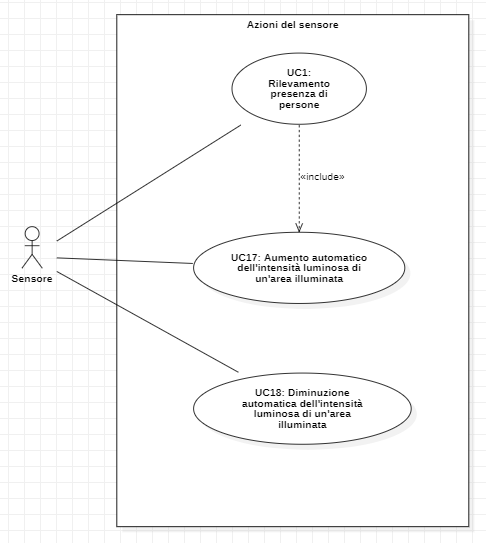
\includegraphics[scale=0.7]{diagramma_use_case_1.png}

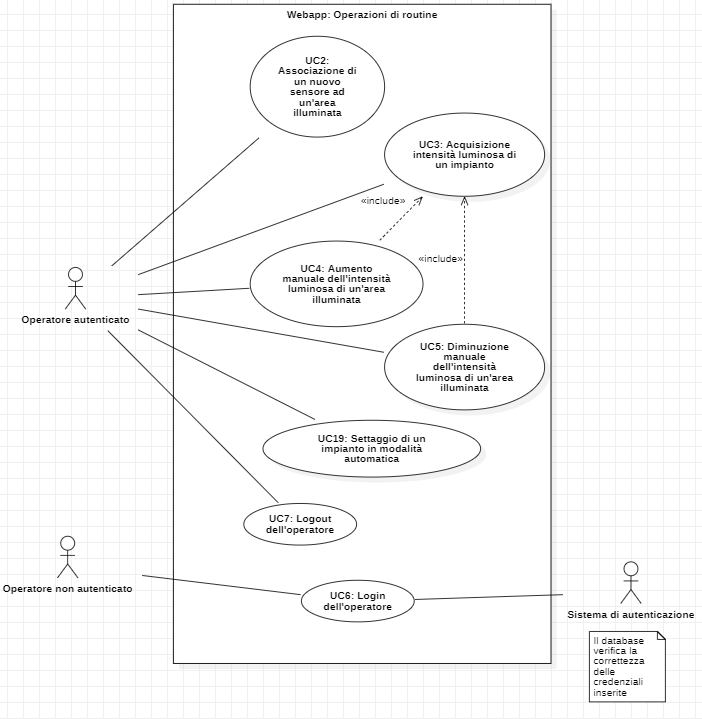
\includegraphics[scale=0.65]{diagramma_use_case_2.png}

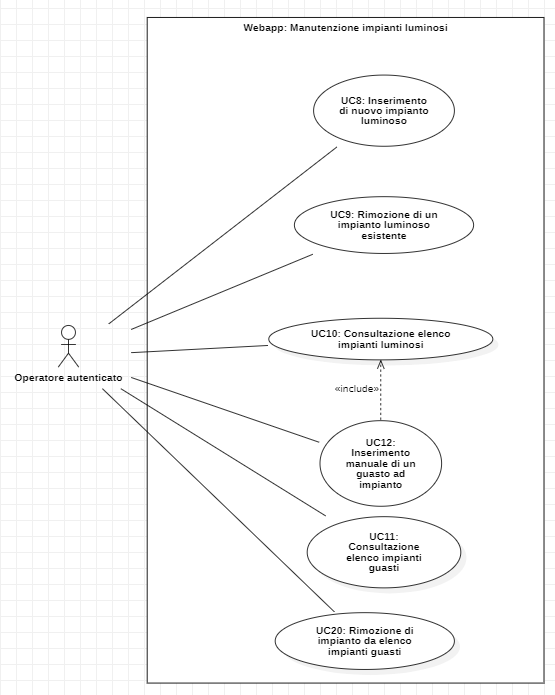
\includegraphics[scale=0.7]{diagramma_use_case_3.png}

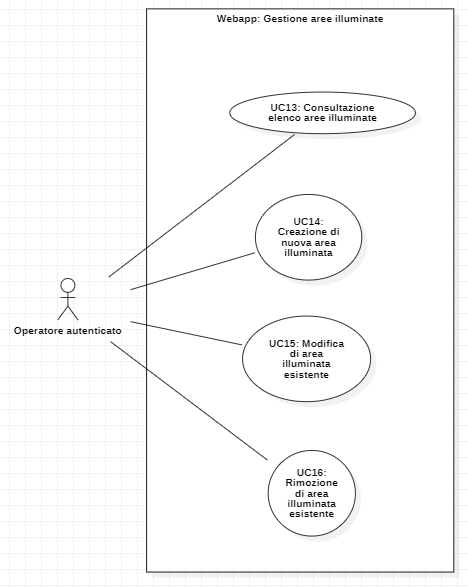
\includegraphics[scale=0.7]{diagramma_use_case_4.png}

\subsection{Attori}
\begin{itemize}
    \item Operatore non autenticato: operatore che non ha inserito le proprie credenziali;
    \item Operatore autenticato: operatore che ha inserito correttamente le credenziali;
    \item Sistema di autenticazione: sistema di controllo che permette di verificare il corretto inserimento dei dati per accedere al programma;
    \item Sistema di gestione dell'illuminazione: sistema di controllo per la
    manipolazione dei dati relativi alle aree illuminate.
\end{itemize}

\subsection{Lista dei casi d'uso}
\subsubsection{UC1 - Rilevamento presenza di persone}
\textbf{Attore:} sensore.\newline
\textbf{PRE:} l'individuo non è ancora posizionato in prossimità dell'area con lampioni, i lampioni sono spenti.\newline
\textbf{POST:} l'individuo è posizionato all'interno dell'area, i lampioni illuminano l'area.\newline
\textbf{Scenario principale:}
\begin{enumerate}
    \item Il sensore rileva la presenza di uno o più individui nel raggio d'azione;
    \item Il sistema riceve in modalità push/pull le informazioni dal sensore;
    \item Il sistema elabora l'informazione ricevuta, aumenta l'intensità luminosa dell'area (include[UC17]) per un certo tempo;
    \item A seguire, l'intensità luminosa dell'area viene riportata al valore di default.
\end{enumerate}

\subsubsection{UC2 - Associazione di un nuovo sensore ad un'area illuminata}
\textbf{Attore:} operatore autenticato.\newline
\textbf{PRE:} il sensore è fisicamente presente in un'area, ma non è configurato per essere parte del sistema gestito dall'applicazione.\newline
\textbf{POST:} il sensore è inserito nel sistema ed è raggiungibile.\newline
\textbf{Scenario principale:}
\begin{enumerate}
    \item L'operatore accede al sistema;
    \item L'operatore effettua il login con proprie credenziali;
    \item L'operatore avvia procedura inserimento;
    \item L'operatore specifica tipo di interazione push/pull, dettagli, posizione geografica dispositivo, raggio d'azione;
    \item L'operatore specifica l'area illuminata di riferimento;
    \item Viene ottenuta la conferma dell'inserimento.
\end{enumerate}

\subsubsection{UC3 - Acquisizione intensità luminosa di un impianto}
\textbf{Attore:} operatore autenticato.\newline
\textbf{PRE:} un'area luminosa configurata illumina con un intensità iniziale arbitraria.\newline
\textbf{POST:} l'area luminosa summenzionata illumina con una precisa intensità finale.\newline
\textbf{Scenario principale:}
\begin{enumerate}
    \item L'operatore accede al sistema;
    \item L'operatore effettua il login con proprie credenziali;
    \item Il sistema acquisisce l'elenco di tutte le aree illuminate;
    \item L'operatore seleziona una o più aree illuminate;
    \item L'operatore imposta un valore di intensità luminosa per tutti gli impianti nelle aree selezionate in 4;
    \item Il sistema configura tutti gli impianti selezionati in 4. all'intensità selezionata in 5.
\end{enumerate}

\subsubsection{UC4 - Aumento manuale dell'intensità luminosa di un'area illuminata}
\textbf{Attore:} operatore autenticato.\newline
\textbf{PRE:} un'area luminosa configurata illumina con un intensità iniziale arbitraria.\newline
\textbf{POST:} l'area luminosa summenzionata illumina con una precisa intensità finale.\newline
\textbf{Scenario principale:}
\begin{enumerate}
    \item L'operatore accede al sistema;
    \item L'operatore effettua il login con proprie credenziali;
    \item Il sistema mostra elenco di tutte le aree illuminate;
    \item L'operatore seleziona una o più aree illuminate;
    \item L'operatore imposta un valore maggiore di intensità luminosa per tutti gli impianti nelle aree selezionate in 4;
    \item Il sistema configura tutti gli impianti selezionati in 4. all'intensità selezionata in 5.
\end{enumerate}

\subsubsection{UC5 - Diminuzione manuale dell'intensità luminosa di un'area illuminata}
\textbf{Attore:} operatore autenticato.\newline
\textbf{PRE:} un'area luminosa configurata illumina con un intensità iniziale arbitraria.\newline
\textbf{POST:} l'area luminosa summenzionata illumina con una precisa intensità finale.\newline
\textbf{Scenario principale:}
\begin{enumerate}
    \item L'operatore accede al sistema;
    \item L'operatore effettua il login con proprie credenziali;
    \item Il sistema mostra elenco di tutte le aree illuminate;
    \item L'operatore seleziona una o più aree illuminate;
    \item L'operatore imposta un valore minore di intensità luminosa per tutti gli impianti nelle aree selezionate in 4;
    \item Il sistema configura tutti gli impianti selezionati in 4. all'intensità selezionata in 5.
\end{enumerate}

\subsubsection{UC6 - Login di un operatore}
\textbf{Attore:} operatore non autenticato.\newline
\textbf{PRE:} l'operatore non è entrato nel sistema e quindi non può gestire i sistemi di illuminazione, ma è registrato nel database.\newline
\textbf{POST:} l'operatore ha inserito le proprie credenziali e può gestire i sistemi di illuminazione.\newline
\textbf{Scenario principale:}
\begin{enumerate}
    \item L'operatore accede al sistema;
    \item L'operatore inserisce le proprie credenziali;
    \item Il sistema verifica se le credenziali corrispondono a quelle di un utente nel database;
\end{enumerate}
\textbf{Estensioni:}
\begin{itemize}
    \item [a.] Le credenziali inserite non sono corrette;
    \begin{enumerate}
        \item Viene visualizzato un errore;
        \item L'operatore deve immettere nuovamente le proprie credenziali.
    \end{enumerate}
\end{itemize}

\subsubsection{UC7 - Logout dell'operatore}
\textbf{Attore:} operatore autenticato.\newline
\textbf{PRE:} l'operatore ha il consenso di gestire i sistemi di illuminazione tramite l'applicazione.\newline
\textbf{POST:} all'operatore non è consentito gestire i sistemi di illuminazione tramite l'applicazione, ma è registrato nel database.\newline
\textbf{Scenario principale:}
\begin{enumerate}
    \item L'operatore ha l'accesso del sistema;
    \item L'operatore seleziona il pulsante di Logout;
    \item L'applicazione termina la sessione dell'operatore;
\end{enumerate}

\subsubsection{UC8 - Inserimento di nuovo impianto luminoso}
\textbf{Attore:} operatore autenticato.\newline
\textbf{PRE:} l'impianto è fisicamente presente ma non è registrato nel sistema.\newline
\textbf{POST:} l'impianto è stato registrato correttamente e sarà possibile gestirlo tramite applicazione.\newline
\textbf{Scenario principale:}
\begin{enumerate}
    \item L'operatore accede al sistema;
    \item L'operatore effettua il login con proprie credenziali;
    \item L'operatore avvia procedura inserimento;
    \item L'operatore specifica il sensore che gestirà l'impianto e i relativi dettagli;
    \item Viene ottenuta la conferma dell'inserimento.
\end{enumerate}

\subsubsection{UC9 - Rimozione di un impianto luminoso esistente}
\textbf{Attore:} operatore autenticato.\newline
\textbf{PRE:} l'impianto è registrato nel sistema.\newline
\textbf{POST:} l'impianto è stato cancellato dal database e non sarà possibile gestirlo dall'applicazione.\newline
\textbf{Scenario principale:}
\begin{enumerate}
    \item L'operatore accede al sistema;
    \item L'operatore effettua il login con proprie credenziali;
    \item L'operatore avvia procedura di rimozione;
    \item Viene visualizzato l'elenco degli impianti luminosi esistenti;
    \item L'operatore seleziona l'impianto da rimuovere dal sistema;
    \item Viene chiesta la conferma di eliminazione;
    \item L'operatore conferma l'operazione;
    \item Viene rimosso l'impianto luminoso dal sistema;
    \item Viene ottenuta la conferma di rimozione.
\end{enumerate}
\textbf{Estensioni:}
\begin{itemize}
    \item [a.] L'operatore non conferma la rimozione alla richiesta di conferma;
    \begin{enumerate}
        \item Viene visualizzato l'elenco degli impianti luminosi esistenti;
        \item L'operatore devrà selezionare un impianto da eliminare o annullare la procedura;
    \end{enumerate}
    \item [b.] Viene annullata la procedura di rimozione;
    \begin{enumerate}
        \item La lista degli impianti non subisce modifiche;
        \item Viene visualizzata la schermata principale.
    \end{enumerate}
\end{itemize}

\subsubsection{UC10 - Consultazione elenco impianti luminosi}
\textbf{Attore:} operatore autenticato.\newline
\textbf{PRE:} l'operatore non visualizza l'elenco degli impianti luminosi.\newline
\textbf{POST:} l'operatore visualizza l'elenco degli impianti e potrà interagire con esso.\newline
\textbf{Scenario principale:}
\begin{enumerate}
    \item L'operatore accede al sistema;
    \item L'operatore effettua il login con proprie credenziali;
    \item L'operatore seleziona il pulsante di consultazione elenco impianti luminosi;
    \item Viene visualizzato l'elenco degli impainti luminosi.
\end{enumerate}

\subsubsection{UC11 - Consultazione elenco impianti guasti}
\textbf{Attore:} operatore autenticato.\newline
\textbf{PRE:} l'operatore non visualizza l'elenco degli impianti con segnalato dei guasti.\newline
\textbf{POST:} l'operatore consulta l'elenco degli impianti dei guasti e interagisce con esso.\newline
\textbf{Scenario principale:}
\begin{enumerate}
    \item L'operatore accede al sistema;
    \item L'operatore effettua il login con proprie credenziali;
    \item L'operatore seleziona il pulsante di consultazione elenco impianti guasti;
    \item Viene visualizzato l'elenco degli impianti guasti.
\end{enumerate}

\subsubsection{UC12 - Inserimento manuale di un guasto ad un impianto}
\textbf{Attore:} operatore autenticato.\newline
\textbf{PRE:} è presente un impianto non funzionante che non è incluso nella lista degli impianti guasti.\newline
\textbf{POST:} l'impianto non funzionante è incluso nella lista degli impianti guasti.\newline
\textbf{Scenario principale:}
\begin{enumerate}
    \item L'operatore accede al sistema;
    \item L'operatore effettua il login con proprie credenziali;
    \item L'operatore avvia la procedura per l’inserimento di un impianto luminoso guasto;
    \item Viene consultato l’elenco degli impianti di illuminazione attivi(include [UC10]).
    \item L'operatore marca il dispositivo interessato come guasto, scatenandone l’inserimento dell’elenco degli impianti di illuminazione guasti.
\end{enumerate}

\subsubsection{UC13 - Consultazione elenco aree illuminate}
\textbf{Attore:} operatore autenticato.\newline
\textbf{PRE:} l'operatore non visualizza l'elenco delle aree illuminate.\newline
\textbf{POST:} l'operatore visualizza l'elenco delle aree illuminate e potrà interagire con esso.\newline
\textbf{Scenario principale:}
\begin{enumerate}
    \item L'operatore accede al sistema;
    \item L'operatore effettua il login con proprie credenziali;
    \item L'operatore seleziona il pulsante di consultazione elenco aree illuminate;
    \item Viene visualizzato l'elenco delle aree illuminate.
\end{enumerate}

\subsubsection{UC14 - Creazione di nuova area illuminata}
\textbf{Attore:} operatore autenticato.\newline
\textbf{PRE:} l'area illuminata non è presente nel sistema.\newline
\textbf{POST:} l'area illuminata è presente nel sistema ed è possibile gestirla tramite applicazione.\newline
\textbf{Scenario principale:}
\begin{enumerate}
    \item L'operatore accede al sistema;
    \item L'operatore effettua il login con proprie credenziali;
    \item L'operatore avvia la procedura di creazione di una nuova area illuminata;
    \item L'operatore specifica posizione geografica e relativi dettagli;
    \item Viene ottenuta la conferma di inserimento.
\end{enumerate}

\subsubsection{UC15 - Modifica di area illuminata esistente}
\textbf{Attore:} operatore autenticato.\newline
\textbf{PRE:} l'area illuminata è registrata con dati arbitrari.\newline
\textbf{POST:} l'area illuminata è registrata con i dati aggiornati.\newline
\textbf{Scenario principale:}
\begin{enumerate}
    \item L'operatore accede al sistema;
    \item L'operatore effettua il login con proprie credenziali;
    \item L'operatore avvia la procedura di modifica di un'area illuminata;
    \item Viene visualizzato l'elenco delle aree illuminate;
    \item L'operatore selezione l'area illuminata che desidera modificare;
    \item Viene visualizzata la schermata di modifica dell'area illuminata selezionata in 5;
    \item L'operatore modifica l'area illuminata con dati aggiornati;
    \item Viene ottenuta la conferma di modifica.
\end{enumerate}

\subsubsection{UC16 - Rimozione di area illuminata esistente}
\textbf{Attore:} operatore autenticato.\newline
\textbf{PRE:} l'area illuminata è presente nel sistema e visibile tramite applicazione.\newline
\textbf{POST:} l'area illuminata non è presente nel sistema.\newline
\textbf{Scenario principale:}
\begin{enumerate}
    \item L'operatore accede al sistema;
    \item L'operatore effettua il login con proprie credenziali;
    \item L'operatore avvia la procedura di rimozione di un'area illuminata;
    \item Viene visualizzato l'elenco delle aree illuminate esistenti;
    \item L'operatore selezione l'area illuminata che desidera rimuovere;
    \item Viene visualizzata la richiesta di conferma di cancellazione;
    \item L'operatore conferma l'operazione;
    \item Viene rimossa l'area illuminata dal sistema;
    \item Viene ottenuta la conferma di rimozione.
\end{enumerate}
\textbf{Estensioni:}
\begin{itemize}
    \item [a.] L'operatore non conferma la rimozione alla richiesta di conferma:
    \begin{enumerate}
        \item Viene visualizzato l'elenco delle aree illuminate esistenti;
        \item L'operatore dovrà selezionare un'area illuminata da eliminare o annullare la procedura;
    \end{enumerate}
    \item [b.] Viene annullata la procedura di rimozione:
    \begin{enumerate}
        \item La lista delle aree illuminate non subisce modifiche;
        \item Viene visualizzata la schermata principale.
    \end{enumerate}
\end{itemize}

\subsubsection{UC17 - Aumento automatico dell'intensità luminosa di un'area illuminata}
\textbf{Attori:}
\begin{itemize}
    \item sensore;
    \item sistema di gestione dell'illuminazione.
\end{itemize}
\textbf{PRE:} un'area luminosa configurata illumina con un'intensità iniziale arbitraria.\newline
\textbf{POST:} l'area luminosa summenzionata illumina con una precisa intensità finale.\newline
\textbf{Scenario principale:}
% DA CONTROLLARE: Non è il sensore che modifica l'intensità, ma esso fornisce il
% l'informazione al software del passaggio della persona: poi il software
% automaticamente aumenta la luminosità.
\begin{enumerate}
    \item Il sensore rileva la presenza di persone in una area illuminata precisa; [UC1]
    \item Il sistema di gestione dell'illuminazione aumenta l'intensità luminosa dell'area illuminata rilevata in 1.
\end{enumerate}

\subsubsection{UC18 - Diminuzione automatica dell'intensità luminosa di un'area illuminata}
\textbf{Attori:}
\begin{itemize}
    \item sensore;
    \item sistema di gestione dell'illuminazione.
\end{itemize}
\textbf{PRE:} un'area luminosa configurata illumina con un'intensità iniziale arbitraria.\newline
\textbf{POST:} l'area luminosa summenzionata illumina con una precisa intensità finale.\newline
\textbf{Scenario principale:}
% DA CONTROLLARE: Non è il sensore che modifica l'intensità, ma esso fornisce il
% l'informazione al software della mancata presenza della persona: poi il software
% automaticamente diminuisce la luminosità.
\begin{enumerate}
    \item Il sensore rileva che in un'area illuminata con intensità luminosa alta non ci sono persone presenti;
    \item il sistema di gestione dell'illuminazione diminuisce l'intensità luminosa dell'area illuminata rilevata in 1.
\end{enumerate}

\subsubsection{UC19 - Settaggio di un impianto in modalità automatica}
\textbf{Attore:} operatore autenticato.\newline
\textbf{PRE:} l'impianto non è stato settato con modalità automatica.\newline
\textbf{POST:} l'impianto ha la modalità automatica attiva e può gestire i dispositivi collegati ad esso.\newline
\textbf{Scenario principale:}
\begin{enumerate}
    \item L'operatore accede al sistema;
    \item L'operatore effettua il login con proprie credenziali;
    \item L'operatore avvia la procedura di settaggio di un impianto in modalità automatica;
    \item L'operatore visualizza l'elenco degli impianti esistenti;
    \item L'operatore seleziona l'impianto che desidera impostare con modalità automatica;
    \item Viene ottenuta la conferma di attivazione della modalità automatica dell'impianto selezionato in 5.
\end{enumerate}

\subsubsection{UC20 - Rimozione di impianto da elenco impianti guasti}
\textbf{Attore:} operatore autenticato.\newline
\textbf{PRE:} l'impianto è presente nel sistema come impianto guasto.\newline
\textbf{POST:} l'impianto è presente nel sistema ma viene indicato come impianto
attivo e non più come impianto guasto.\newline
\textbf{Scenario principale:}
% DA CONTROLLARE: ultimo pezzo modificato da verificare
\begin{enumerate}
    \item L'operatore accede al sistema;
    \item L'operatore effettua il login con proprie credenziali;
    \item L'operatore avvia la procedura di rimozione di un impianto guasto;
    \item Viene visualizzato l'elenco degli impianti guasti esistenti;
    \item L'operatore seleziona l'impianto che desidera rimuovere dall'elenco;
    \item Viene ottenuta la conferma di rimozione;
    \item L'impianto ritorna nella lista degli impianti attivi.
\end{enumerate}

\newpage
\section{Requisiti}
Ogni requisito è identificato da un codice la cui struttura è definita nelle \textit{Norme di Progetto}.
\subsection{Requisiti funzionali}
%R+tipologia(F/Q/V)+caso d'uso relativo.sottocaso - importanza (O/D/F) 
\setlength\tabcolsep{4pt}
\begin{longtable}{|c|p{7cm}|c|p{4cm}|}
    \hline
    \multicolumn{4}{| c |}{\textbf{Requisiti funzionali}} \\
    \hline
    \textbf{Codice} & \textbf{Descrizione} & \textbf{Rilevanza} & \textbf{Fonti} \\
    \hline
    RF1-O & Rilevamento della presenza di individui in una delle aree illuminate. & Obbligatorio & UC1 \\
    \hline
    RF2-O & Inserimento di un nuovo sensore presente in un'area ma non ancora inserito per essere gestito dal sistema. & Obbligatorio & UC2 \\
    \hline
    RF3-O & Acquisizione dell'intensità luminosa e successiva determinazione precisa del livello di luminosità. & Obbligatorio & UC3 \\    
    \hline
    RF4-O & Una volta acquisito il livello di luminosità iniziale, l'operatore autenticato aumenta manualmente il livello di intesità luminosa. & Obbligatorio & UC4 \\    
    \hline
    RF5-O & Una volta acquisito il livello di luminosità iniziale, l'operatore autenticato diminuisce manualmente il livello di intensità luminosa. & Obbligatorio & UC5 \\    
    \hline
    RF6-O & Il gestore può effettuare l'accesso per gestire manualmente i sistemi di illuminazione. & Obbligatorio & UC6 \\    
    \hline
    RF7-O & Il gestore può effettuare il logout dall'interno dell'area di gestione dei sistemi. & Obbligatorio & UC7 \\
    \hline
    RF8-O & Il gestore può inserire nel sistema l'impianto da attivare con i
    relativi dettagli. & Obbligatorio & UC8\\
    \hline
    RF9-O & Il gestore può rimuovere dal sistema uno degli impianti luminosi
    registrati. & Obbligatorio & UC9 \\
    \hline
    RF10-O & Il gestore può consultare l'intero elenco degli impianti attivi. & Obbligatorio & UC10 \\
    \hline
    RF11-O & Il gestore può consultare l'intero elenco degli impianti guasti. & Obbligatorio & UC11 \\
    \hline
    RF12-O & Il gestore può aggiungere manualmente un guasto selezionando un
    impianto dalla lista di quelli attivi. & Obbligatorio & UC12 \\
    \hline
    RF13-O & Il gestore può consultare l'elenco delle aree illuminate. & Obbligatorio & UC13 \\
    \hline
    RF14-O & Il gestore può creare una nuova area illuminata, inserendone la
    posizione geografica e i relativi dettagli. & Obbligatorio & UC14 \\
    \hline
    RF15-O & Il gestore può modificare i dettagli di un'area illuminata già esistente. & Obbligatorio & UC15 \\
    \hline
    RF16-O & Il gestore può rimuovere un'area illuminata già esistente. &
    Obbligatorio & UC16 \\
    \hline
    RF17-O & Il sistema di gestione dell'illuminazione aumenta l'intensità
    luminosa al passaggio di una o più persone. & Obbligatorio & UC17 \\
    \hline
    RF18-O & Il sistema di gestione dell'illuminazione diminuisce l'intensità
    luminosa al passaggio di una o più persone. & Obbligatorio & UC18 \\
    \hline
    RF19-O & Il gestore può impostare la modalità di funzionamento automatico
    per l'impianto selezionato. & Obbligatorio & UC19 \\
    \hline
    RF20-O & Il gestore può rimuovere un impianto dall'elenco degli impianti
    guasti e ritorna negli impianti attivi. & Obbligatorio & UC20 \\
    \bottomrule
\end{longtable}
\end{document}